	\newpage
\section{Implementacja}		%4
%Wkleić szkielet kodu, wraz z komentarzami. Opisać zmienne, struktury do czego służą. Opisać procedury, metody co wykonują. Opisać nowe zdefiniowane klasy. Opisać dziedziczenie. Opisać nowo utworzone pliki za co odpowiadają.
\hspace{1cm} \textbf{Tworznie Menu:} \newline 
Do stworzenia menu użyty został \textbf{Xamarin.forms Shell}, który zmiejsza złożoność tworzenia aplikacji, oferując podstawowe funkcje. Obejmuje on wspólne środowisko użytkownika nawigacji, schematu nawigacji i zintegrowanej procedury obsługi wyszukiwania.
\newline
\newline
\textbf{Dodawanie strony do menu na przykładzie elementu wyniki:}
\newline
W pliku \textbf{MainPage.xaml}:
\newline
\newline
\begin{figure}[!htb]
	\begin{center}
		\includegraphics[width=12cm]{rys/item.png}
		\caption{Dodanie strony Menu do menu bocznego}
		\label{rys:rysunek012}
	\end{center}
\end{figure}
\newline
Na rysunku 4.1 \textbf{ic\_wyniki} to nazwa ikonki a \textbf{local:Wyniki} to odnośnik do plików strony "Wyniki", które znajdują się w folderze głównym projektu. 
\newline
\newline
\textbf{Dodawanie ikonek do projektu:} \newline
Ikonki pobrane zostały z \textbf{Android Asset Studio} w formacie ".png". \newline
Aby użyć ikonki w projekcie należy umieścić je w dwóch osobnych miejscach. Dla androida jest to folder \textbf{drawable} znajdujący się w folderze resources a dla systemu iOS folder \textbf{resources}.
\newline \newline
\newpage
Działanie menu bocznego w emulatorze Android 8.1:
\begin{figure}[!htb]
	\begin{center}
		\includegraphics[width=6cm]{rys/ZSmenu.png}
		\caption{Widok menu bocznego}
		\label{rys:rysunek013}
	\end{center}
\end{figure}

Na rysunku 4.2 można zobaczyć menu boczne z opcjami do wyboru.


\begin{figure}[!htb]
	\begin{center}
		\includegraphics[width=5cm]{rys/ZSotwartastrona.png}
		\caption{Widok strony otwartej po wybraniu danej opcji z menu}
		\label{rys:rysunek014}
	\end{center}
\end{figure}

Na rysunku 4.3 widzimy nowo otwartą stronę po wybraniu opcji z menu bocznego.

 \textbf{Dodanie pól wyboru na stronie "Wybierz normę":} \newline
 Do stworzenia pól wyboru z których można wybrąć tylko jedną opcję potrzebne jest zainstalowanie pakietu Nuget \textbf{Xamarin.Forms.InputKit}. Przy użyciu tego pakietu można użyć opcji \textbf{RadioButton}, dzięki której tworzona jest lista z polami do wyboru. \newline \newline
 Fragment kodu z pliku \textbf{Wybierz\_norme.xml} został pokazany na rysunku 4.4. \newline
 \begin{figure}[!htb]
 	\begin{center}
 		\includegraphics[width=12cm]{rys/checkboxy.png}
 		\caption{Dodanie opcji z polami do wyboru}
 		\label{rys:rysunek015}
 	\end{center}
 \end{figure}
 

 \textbf{Dodanie mapy pokazującej obecną lokalizację}
 \newline
 Użycie pakietu Nuget xamarin.forms.maps umożliwia wyświetlenie na stronie mapy ze znacznikiem pokazującym obecną lokalizacje.
 \newline 
 W pliku \textbf{AndroidManifest.xml} w sekcji application - meta-data należy dodać klucz interfejsu API, który można utworzyć na stronie \textbf{developers.google.com}. Wprowadzić należy także nazwe metadanych dla klucza intefejsu API.
 Kolejna linijka również posiada sekcję meta-data i określa numer wersji Google Play usługi. W sekcji uses-library deklarowana jest biblioteka Apache HTTP jak to zostało pokazane na rysunku 4.5.

 \begin{figure}[!htb]
 	\begin{center}
 		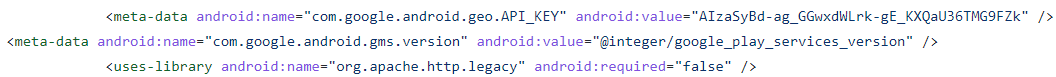
\includegraphics[width=15cm]{rys/map_manifest.png}
 		\caption{Dodanie nowych deklaracji w AndroidManifest.xaml}
 		\label{rys:rysunek016}
 	\end{center}
 \end{figure}
 
 Na rysunku 4.6 widzimy fragment pliku \textbf{mapa.xaml.cs} w którym utworzona została klasa \textbf{DisplayCurLoc}, w której zawarte są instrukcje odpowiedzialne za wykrycie obecnej lokalizacji.
 \newline
 \newline
 \begin{figure}[!htb]
 	\begin{center}
 		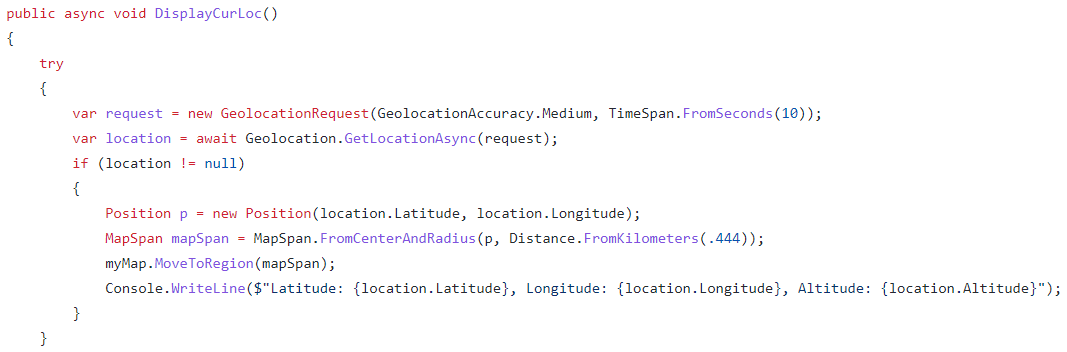
\includegraphics[width=15cm]{rys/mapa_xaml_cs.png}
 		\caption{Dodanie funkcji w mapa.xaml.cs}
 		\label{rys:rysunek017}
 	\end{center}
 \end{figure}
 
 W pliku \textbf{mapa.xaml} wartość opcji IsShowingUser ustawiona jest jako True, dzięki czemu na mapie wyświetlony zostanie znacznik wskazujący na obecną lokalizację. Opcja x:Name nadaje nazwę dla używanej mapy tak jak na rysunku 4.7.
 \newline
\begin{figure}[!htb]
	\begin{center}
		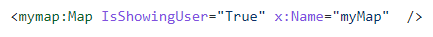
\includegraphics[width=8cm]{rys/mapa_xaml.png}
		\caption{Ustawienie opcji w mapa.xaml}
		\label{rys:rysunek018}
	\end{center}
\end{figure}
   

\textbf{Dodanie obsługi aparatu} \newline
Do obsługi aparatu użyty został pakiet Nuget \textbf{Xam.Plugin.Media}. Po naciśnięciu przycisku otwiera się aparat telefonu i można wykonać zdjęcie, które następnie zostanie zapisane i wyświetlone na stronie.
\newline
\begin{figure}[!htb]
	\begin{center}
		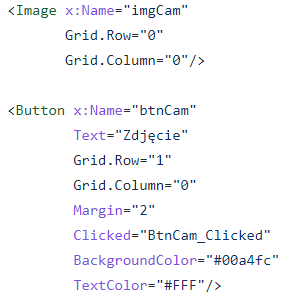
\includegraphics[width=4cm]{rys/Zdjecia_xaml.png}
		\caption{Plik Zdjecia.xml}
		\label{rys:rysunek019}
	\end{center}
\end{figure}
\newline
Na rysunku 4.8 przedstawiony jest fragment kodu ze strony \textbf{Zdjecia.xml}. Opcja Image odpowiada za dodanie zrobionego zdjęcia na stronę. Opcja Button tworzy przycisk z napisem Zdjęcie, którego naciśnięcie otworzy aparat.

\begin{figure}[!htb]
	\begin{center}
		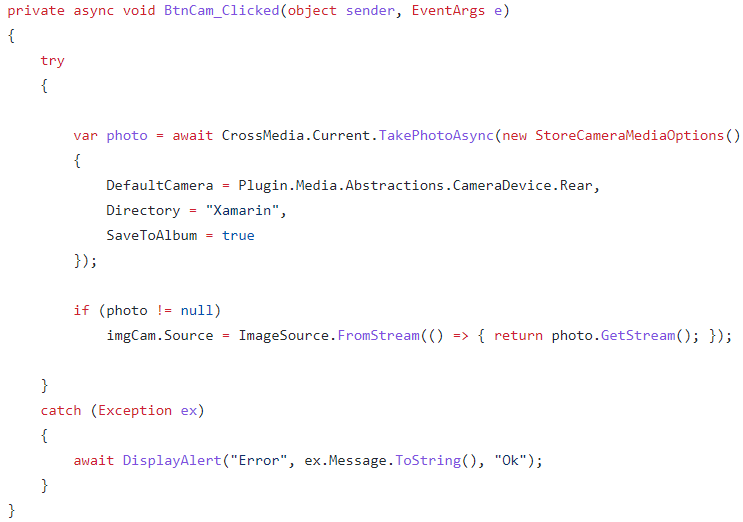
\includegraphics[width=12cm]{rys/Zdjecia_xaml_cs.png}
		\caption{Plik Zdjecia.xml.cs}
		\label{rys:rysunek020}
	\end{center}
\end{figure}

Na rysunku 4.9 znajduje się fragment kodu znajdującego się na stronie \textbf{Zdjecia.xml.cs}. Funkcja \textbf{BtnCamClicked} ustawia domyślną kamerę na tylną kamerę naszego telefonu. Ścieżka pliku obrazu ustawiona jest do folderu "Xamarin". Atrybut zostaje przekazany jako true, aby zapisać obraz.
  
\begin{figure}[!htb]
	\begin{center}
		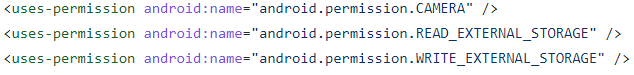
\includegraphics[width=12cm]{rys/Zdjecia_manifest.png}
		\caption{Plik AndroidManifest.xml}
		\label{rys:rysunek021}
	\end{center}
\end{figure}  

Na rysunku 4.10 przedstawiony jest fragment pliku \textbf{AndroidManifest.xml}. Aby prawidłowa obsługa aparatu była możliwa zadeklarowane muszą być zezwolenia na dostęp do uprawnień aparatu i pamięci zewnętrznej. \newline \newline

\textbf{Rejestracja i logowanie z wykorzystaniem Google Firebase} \newline
Baza danych Google Firebase umożliwia rejestrację oraz logowanie użytkowników do aplikacji. Użytkownicy, którzy utworzą nowe konto zostają zapisani w bazie danych i mają możliwość logowania się do aplikacji za pomocą adresu Email i hasła\footnote{https://firebase.google.com/docs/auth\cite{www3}.}. \newline
Do korzystania z autoryzacji Firebase konieczne jest pobranie dwóch pakietów Nuget: \textbf{Xamarin.Firebase.Auth} i \textbf{Xamarin.Firebase.Core} oraz inicjalizacja usługi w pliku \textbf{MainActivity.cs} w rozwiązaniu Android co zostało pokazane na rysunku 4.11.

\begin{figure}[!htb]
	\begin{center}
		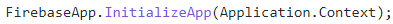
\includegraphics[width=12cm]{rys/firebase_main_activity.png}
		\caption{Inicjalizacja w pliku MainActivity.cs}
		\label{rys:rysunek022}
	\end{center}
\end{figure}

W rozwiązaniu głównym  stworzony został plik \textbf{Iauth.cs} a w nim interfejs \textbf{Iauth}.
 
 \begin{figure}[!htb]
 	\begin{center}
 		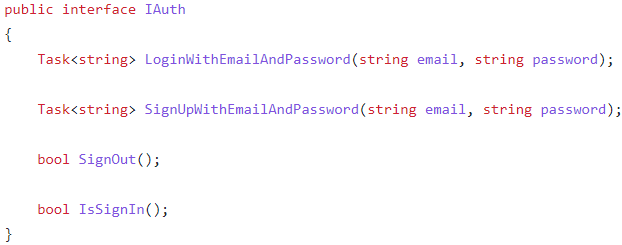
\includegraphics[width=14cm]{rys/iauth.png}
 		\caption{Interfejs Iauth w pliku Iauth.cs}
 		\label{rys:rysunek023}
 	\end{center}
 \end{figure}

Jak widać na rysunku 4.12 wewnątrz interfejsu utworzone zostały cztery funkcje. \textbf{LoginwithEmailAndPassword}  i \textbf{SignUpWithEmailAndPassword}, które przyjmują email i hasło jako zmienne typu string i będą wykorzystywane przy tworzeniu nowego konta a także przy logowaniu. Funkcje bool \textbf{SignOut} oraz \textbf{IsSignIn} bedą potrzebne do sprawdzania statusu użytkownika. \newline \newline 

W rozwiązaniu dla Androida utworzono klasę \textbf{AuthDroid.cs} w której znajdują się instrukcję dla funkcji, które zostały pokazane w interfejsie. 

\begin{figure}[!htb]
	\begin{center}
		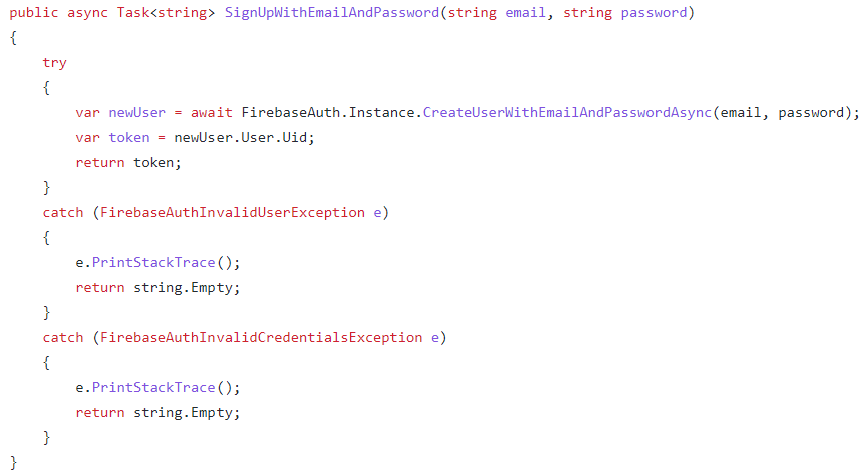
\includegraphics[width=15cm]{rys/authdroid1.png}
		\caption{Funkcja rejestracji}
		\label{rys:rysunek024}
	\end{center}
\end{figure}

Na rysunku 4.13 przedstawiono funkcję rejestracji. Przy użyciu autoryzacji Firebase torzone jest nowe konto użytkownika. Pobrany zostaje Email i hasło a użytkownik otrzymuje unikalny numer Uid. Aby konto zostało poprawnie utworzone należy użyć poprawnej formy adresu email i hasła o długości minimum 6 znaków. \newline 
Podobnie wygląda to w funkcji odpowiadającej za logowanie przedstawionej na rysunku 4.14. 

\begin{figure}[!htb]
	\begin{center}
		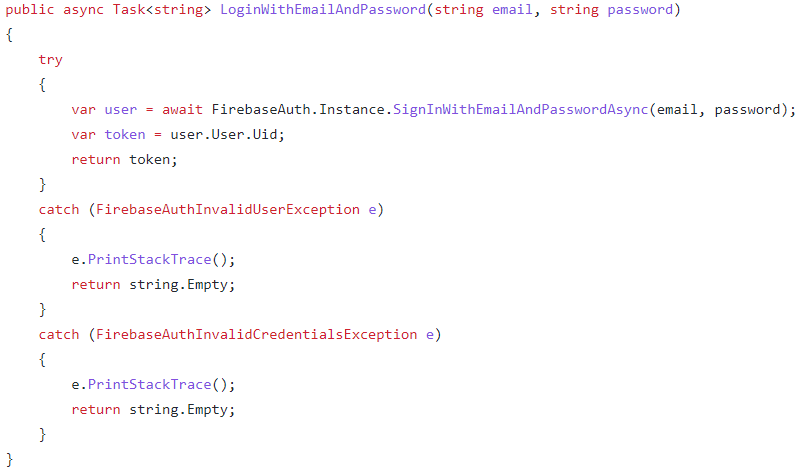
\includegraphics[width=15cm]{rys/authdroid2.png}
		\caption{Funkcja logowania}
		\label{rys:rysunek025}
	\end{center}
\end{figure}

Email i hasło zostają sprawdzone, jeżeli zgadzają się one z danymi zawartymi w bazie to logowanie jest skuteczne. W przypadku użycia błędnych danych użytkownik dostaje informacje o błędzie. \newline \newline

Kolejne dwie funkcje sprawdzają status użytkownika przy użyciu typu bool.

\begin{figure}[!htb]
	\begin{center}
		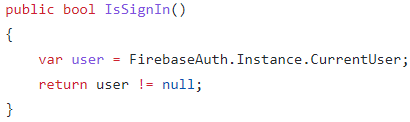
\includegraphics[width=8cm]{rys/authdroid3.png}
		\caption{Funkcja IsSignIn}
		\label{rys:rysunek026}
	\end{center}
\end{figure}  

Widoczna na rysunku 4.15 funkcja \textbf{IsSignIn} sprawdza jaki użytkownik jest zalogowany i zwraca informacje o nim.

\begin{figure}[!htb]
	\begin{center}
		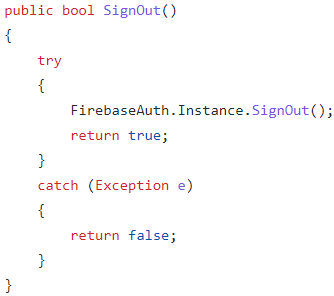
\includegraphics[width=8cm]{rys/authdroid4.png}
		\caption{Funkcja SignOut}
		\label{rys:rysunek027}
	\end{center}
\end{figure}       

Funkcja SignOut widoczna na rysunku 4.16 odpowiada za wylogowanie użytkownika z aplikacji. Jeżeli wszytko przebiegnie prawidłowo zwróci ona wartość true a jeżeli operacja się nie powiedzie to zwróci wartość false. \newline \newline 

W rozwiązaniu głównym w pliku App.xaml dodana jest instrukcja odpowiedzialna za przekierowanie użytkownika. \newline \newline

\begin{figure}[!htb]
	\begin{center}
		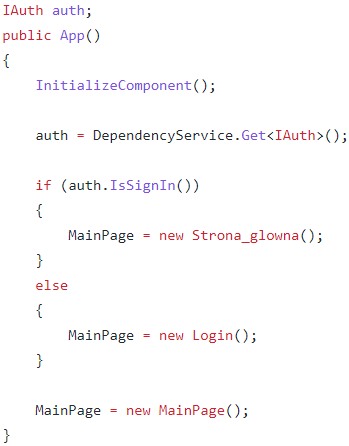
\includegraphics[width=6cm]{rys/firebase_app_xaml.png}
		\caption{Przekierowanie w pliku App.xaml}
		\label{rys:rysunek028}
	\end{center}
\end{figure}

Wywołana zostaje funkcja \textbf{IsSignIn}, która sprawdza czy użytkownik jest poprawnie zalogowany. Jeżeli logowanie przebiegło prawidłowo to użytkownik zostanie przeniesiony na stronę główną aplikacji, natomiast jeżeli logowanie się nie powiedzie to zostaje on przekierowany na strone logowania co widać na rysunku 4.17.   
